Dado que en los sistemas biológicos las partículas se encuentran aleatoriamente orientadas, es de gran utilidad considerar las secciones transversales promedio $\langle C_{abs}\rangle$ y $\langle C_{sca}\rangle$, que son independientes de la polarización de la luz incidente\footnote{Considerando que las partículas no sean ópticamente activas.}, éstas están dadas por \cite{Bohren}
\begin{align*}
	\langle C_{abs}\rangle &= \frac{k}{3} \text{Im}\{\alpha^{(1)}+\alpha^{(2)}+\alpha^{(3)}\},\\
	\langle C_{abs}\rangle &= \frac{k^4}{3(6\pi)} \text{Im}\{\alpha^{(1)}+\alpha^{(2)}+\alpha^{(3)}\}.
\end{align*}

En este trabajo se realizaron los cálculos para elipsoides oblatos, por tanto, se tendrá que por la simetría del elipsoide, $C_{ext}^{(1)}=C_{ext}^{(2)}$ que denotan las secciones transversales de extinción de un elipsoide oblato centrado en el origen con sus semiejes paralelos a los ejes del sistema cartesiano, sobre el cual actúa un campo eléctrico incidente alineado en las direcciones $\hat{e}_x$ y $\hat{e}_y$, respectivamente. En la siguiente figura se grafican $\langle C_{ext}\rangle$, $C_{ext}^{(1)}$ como función de la longitud de onda y de la energía $C_{ext}^{(3)}$ para una partícula de alumino caracterizada por su función dieléctrica dada por el modelo de Drude ($\hbar\omega_p=13.142\text{ eV}$, $\hbar\gamma=0.197\text{ eV}$), con semiejes $a=b=1.5\text{ nm}$, $c=1\text{ nm}$ e inmersa en agua ($n_m=1.33$).

\begin{figure}[h!]
	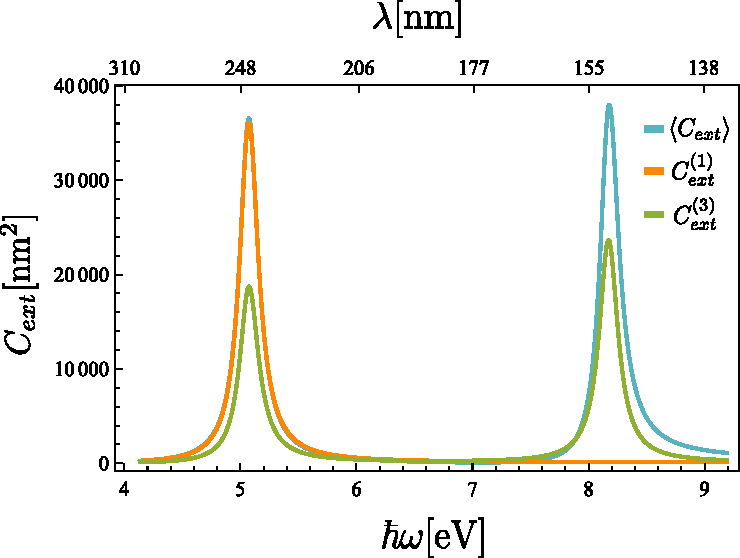
\includegraphics[width=10cm]{../../../../CextAl}
\end{figure}

Dado que se trata de un elipsoide oblato, al considerar $\langle C_{ext}\rangle$ se observan dos resonancias en las que la sección transversal es máxima, que coinciden con las resonancias producto de iluminar a la partícula con un campo eléctrico paralelo a uno de los ejes, dado que se obtiene un promedio, la amplitud de la sección transversal en las resonancias es menor que la de las resonancias individuales.

A continuación se presentan los cálculos de las secciones tranversales de extinción para aluminio, plata, oro, bismuto y óxido de magnesio.

\subsection*{Aluminio y plata}

\subsection*{Oro y bismuto}

\subsection*{Óxido de magnesio}







